%% ---------------------------------------------------------------------------
%% Informe IEEE (Transactions) -- Proyecto de aula, Modelos y Simulación de Sistemas II (UdeA, 2026-2)
%% Clasificación de minerales (cuarzo, pirita, malaquita, hematita) con descriptores clásicos de imagen.
%% Compilar con: pdflatex informe.tex (dos veces).  Clase: IEEEtran [journal] (Overleaf/TeX Live).
%% Las cifras del texto provienen de numeros.tex y las tablas de tablas/*.tex (generados por
%% make_report_assets.py desde los resultados del notebook) para que el texto no pueda desalinearse.
%% ---------------------------------------------------------------------------
\documentclass[journal]{IEEEtran}
\usepackage[utf8]{inputenc}
\usepackage[T1]{fontenc}
\usepackage{mathptmx}
\usepackage[final]{microtype}
\usepackage{amsmath,amssymb}
\usepackage{graphicx}
\usepackage{booktabs}
\usepackage{multirow}
\usepackage{array}
\usepackage{cite}
\usepackage{xcolor}
\usepackage{url}
\makeatletter
% --- idioma: babel-spanish si existe; si no (instalación mínima), nombres a mano + separación silábica propia
\IfFileExists{spanish.ldf}{%
  \usepackage[spanish,es-tabla]{babel}%
  \addto\captionsspanish{\renewcommand{\figurename}{Fig.}\renewcommand{\tablename}{Tabla}%
    \renewcommand{\refname}{Referencias}\renewcommand{\abstractname}{Resumen}}%
}{%
  \renewcommand{\figurename}{Fig.}\renewcommand{\tablename}{Tabla}\renewcommand{\refname}{Referencias}%
  \renewcommand{\abstractname}{Resumen}\IfFileExists{hyph_es.tex}{\input{hyph_es.tex}}{}%
}
\@ifundefined{IEEEabstractname}{}{\renewcommand{\IEEEabstractname}{Resumen}}
\@ifundefined{IEEEkeywordsname}{}{\renewcommand{\IEEEkeywordsname}{Palabras clave}}
\makeatother
% Generado por make_report_assets.py -- NO editar a mano.
\makeatletter
\providecommand{\N}[1]{\@ifundefined{N:#1}{\textbf{??#1??}\PackageWarning{numeros}{Falta la cifra #1}}{\csname N:#1\endcsname}}
\expandafter\gdef\csname N:all-mlp-kstar\endcsname{1835}
\expandafter\gdef\csname N:all-mlp-red\endcsname{0.0}
\expandafter\gdef\csname N:all-mlp-test-acc\endcsname{0.667}
\expandafter\gdef\csname N:all-mlp-test-acc-hi\endcsname{0.80}
\expandafter\gdef\csname N:all-mlp-test-acc-lo\endcsname{0.50}
\expandafter\gdef\csname N:all-mlp-test-f1\endcsname{0.659}
\expandafter\gdef\csname N:all-mlp-test-f1-hi\endcsname{0.80}
\expandafter\gdef\csname N:all-mlp-test-f1-lo\endcsname{0.48}
\expandafter\gdef\csname N:all-mlp-trainf1\endcsname{1.00}
\expandafter\gdef\csname N:all-mlp-val-acc\endcsname{0.626}
\expandafter\gdef\csname N:all-mlp-val-f1\endcsname{0.622}
\expandafter\gdef\csname N:all-mlp-val-f1-ci\endcsname{0.106}
\expandafter\gdef\csname N:all-rf-kstar\endcsname{1835}
\expandafter\gdef\csname N:all-rf-red\endcsname{0.0}
\expandafter\gdef\csname N:all-rf-test-acc\endcsname{0.778}
\expandafter\gdef\csname N:all-rf-test-acc-hi\endcsname{0.88}
\expandafter\gdef\csname N:all-rf-test-acc-lo\endcsname{0.62}
\expandafter\gdef\csname N:all-rf-test-f1\endcsname{0.779}
\expandafter\gdef\csname N:all-rf-test-f1-hi\endcsname{0.90}
\expandafter\gdef\csname N:all-rf-test-f1-lo\endcsname{0.62}
\expandafter\gdef\csname N:all-rf-trainf1\endcsname{1.00}
\expandafter\gdef\csname N:all-rf-val-acc\endcsname{0.834}
\expandafter\gdef\csname N:all-rf-val-f1\endcsname{0.832}
\expandafter\gdef\csname N:all-rf-val-f1-ci\endcsname{0.063}
\expandafter\gdef\csname N:cmt-0-0\endcsname{0.89}
\expandafter\gdef\csname N:cmt-0-1\endcsname{0.00}
\expandafter\gdef\csname N:cmt-0-2\endcsname{0.00}
\expandafter\gdef\csname N:cmt-0-3\endcsname{0.11}
\expandafter\gdef\csname N:cmt-1-0\endcsname{0.22}
\expandafter\gdef\csname N:cmt-1-1\endcsname{0.67}
\expandafter\gdef\csname N:cmt-1-2\endcsname{0.00}
\expandafter\gdef\csname N:cmt-1-3\endcsname{0.11}
\expandafter\gdef\csname N:cmt-2-0\endcsname{0.11}
\expandafter\gdef\csname N:cmt-2-1\endcsname{0.00}
\expandafter\gdef\csname N:cmt-2-2\endcsname{0.89}
\expandafter\gdef\csname N:cmt-2-3\endcsname{0.00}
\expandafter\gdef\csname N:cmt-3-0\endcsname{0.11}
\expandafter\gdef\csname N:cmt-3-1\endcsname{0.22}
\expandafter\gdef\csname N:cmt-3-2\endcsname{0.00}
\expandafter\gdef\csname N:cmt-3-3\endcsname{0.67}
\expandafter\gdef\csname N:cmv-0-0\endcsname{0.85}
\expandafter\gdef\csname N:cmv-0-1\endcsname{0.07}
\expandafter\gdef\csname N:cmv-0-2\endcsname{0.00}
\expandafter\gdef\csname N:cmv-0-3\endcsname{0.08}
\expandafter\gdef\csname N:cmv-1-0\endcsname{0.03}
\expandafter\gdef\csname N:cmv-1-1\endcsname{0.88}
\expandafter\gdef\csname N:cmv-1-2\endcsname{0.02}
\expandafter\gdef\csname N:cmv-1-3\endcsname{0.07}
\expandafter\gdef\csname N:cmv-2-0\endcsname{0.02}
\expandafter\gdef\csname N:cmv-2-1\endcsname{0.08}
\expandafter\gdef\csname N:cmv-2-2\endcsname{0.86}
\expandafter\gdef\csname N:cmv-2-3\endcsname{0.03}
\expandafter\gdef\csname N:cmv-3-0\endcsname{0.17}
\expandafter\gdef\csname N:cmv-3-1\endcsname{0.05}
\expandafter\gdef\csname N:cmv-3-2\endcsname{0.05}
\expandafter\gdef\csname N:cmv-3-3\endcsname{0.74}
\expandafter\gdef\csname N:eda-color-max\endcsname{249}
\expandafter\gdef\csname N:eda-gabor-max\endcsname{13\,927}
\expandafter\gdef\csname N:eda-hu-max\endcsname{30}
\expandafter\gdef\csname N:eda-hu-skew-pct\endcsname{86}
\expandafter\gdef\csname N:eda-n\endcsname{432}
\expandafter\gdef\csname N:eda-p\endcsname{1835}
\expandafter\gdef\csname N:eda-pairs-compact\endcsname{114}
\expandafter\gdef\csname N:eda-pairs-hog\endcsname{332}
\expandafter\gdef\csname N:eda-sd-ratio\endcsname{4\times10^{5}}
\expandafter\gdef\csname N:eda-skew-n\endcsname{764}
\expandafter\gdef\csname N:eda-skew-pct\endcsname{42}
\expandafter\gdef\csname N:ind-cand\endcsname{1130}
\expandafter\gdef\csname N:ind-color-cand\endcsname{3}
\expandafter\gdef\csname N:ind-color-cons\endcsname{15}
\expandafter\gdef\csname N:ind-color-eta\endcsname{0.205}
\expandafter\gdef\csname N:ind-color-etamax\endcsname{0.515}
\expandafter\gdef\csname N:ind-compact-cons\endcsname{37}
\expandafter\gdef\csname N:ind-compact-n\endcsname{71}
\expandafter\gdef\csname N:ind-compact-pct\endcsname{3.9}
\expandafter\gdef\csname N:ind-cons\endcsname{705}
\expandafter\gdef\csname N:ind-gabor-cand\endcsname{11}
\expandafter\gdef\csname N:ind-gabor-cons\endcsname{5}
\expandafter\gdef\csname N:ind-gabor-eta\endcsname{0.203}
\expandafter\gdef\csname N:ind-gabor-etamax\endcsname{0.255}
\expandafter\gdef\csname N:ind-glcm-cand\endcsname{10}
\expandafter\gdef\csname N:ind-glcm-cons\endcsname{10}
\expandafter\gdef\csname N:ind-glcm-eta\endcsname{0.303}
\expandafter\gdef\csname N:ind-glcm-etamax\endcsname{0.399}
\expandafter\gdef\csname N:ind-hog-cand\endcsname{1096}
\expandafter\gdef\csname N:ind-hog-cons\endcsname{668}
\expandafter\gdef\csname N:ind-hog-eta\endcsname{0.042}
\expandafter\gdef\csname N:ind-hog-etamax\endcsname{0.238}
\expandafter\gdef\csname N:ind-hog-pct\endcsname{46}
\expandafter\gdef\csname N:ind-hu-cand\endcsname{6}
\expandafter\gdef\csname N:ind-hu-cons\endcsname{1}
\expandafter\gdef\csname N:ind-hu-eta\endcsname{0.123}
\expandafter\gdef\csname N:ind-hu-etamax\endcsname{0.134}
\expandafter\gdef\csname N:ind-lbp-cand\endcsname{4}
\expandafter\gdef\csname N:ind-lbp-cons\endcsname{6}
\expandafter\gdef\csname N:ind-lbp-eta\endcsname{0.275}
\expandafter\gdef\csname N:ind-lbp-etamax\endcsname{0.322}
\expandafter\gdef\csname N:ind-n-eta02\endcsname{52}
\expandafter\gdef\csname N:ind-n-eta03\endcsname{17}
\expandafter\gdef\csname N:ind-nonsig\endcsname{956}
\expandafter\gdef\csname N:ind-pairs\endcsname{446}
\expandafter\gdef\csname N:ind-pct-cand\endcsname{62}
\expandafter\gdef\csname N:ind-red\endcsname{174}
\expandafter\gdef\csname N:ind-spearman\endcsname{0.51}
\expandafter\gdef\csname N:ind-top-eta\endcsname{0.515}
\expandafter\gdef\csname N:ind-top50-hog\endcsname{3}
\expandafter\gdef\csname N:knn-aug-gain\endcsname{-0.008}
\expandafter\gdef\csname N:knn-aug-gain-ci\endcsname{0.051}
\expandafter\gdef\csname N:knn-aug-sig\endcsname{0}
\expandafter\gdef\csname N:knn-f1-max\endcsname{0.512}
\expandafter\gdef\csname N:knn-f1-min\endcsname{0.473}
\expandafter\gdef\csname N:knn-leak-gap\endcsname{0.044}
\expandafter\gdef\csname N:knn-naive-f1\endcsname{0.556}
\expandafter\gdef\csname N:knn-ncfg\endcsname{16}
\expandafter\gdef\csname N:knn-noaug-f1\endcsname{0.520}
\expandafter\gdef\csname N:knn-test-acc\endcsname{0.472}
\expandafter\gdef\csname N:knn-test-acc-hi\endcsname{0.63}
\expandafter\gdef\csname N:knn-test-acc-lo\endcsname{0.32}
\expandafter\gdef\csname N:knn-test-f1\endcsname{0.460}
\expandafter\gdef\csname N:knn-test-f1-hi\endcsname{0.60}
\expandafter\gdef\csname N:knn-test-f1-lo\endcsname{0.29}
\expandafter\gdef\csname N:knn-train-acc\endcsname{0.74}
\expandafter\gdef\csname N:knn-train-f1\endcsname{0.74}
\expandafter\gdef\csname N:knn-val-acc\endcsname{0.518}
\expandafter\gdef\csname N:knn-val-acc-ci\endcsname{0.071}
\expandafter\gdef\csname N:knn-val-f1\endcsname{0.512}
\expandafter\gdef\csname N:knn-val-f1-ci\endcsname{0.074}
\expandafter\gdef\csname N:lr-aug-gain\endcsname{0.019}
\expandafter\gdef\csname N:lr-aug-gain-ci\endcsname{0.104}
\expandafter\gdef\csname N:lr-aug-sig\endcsname{0}
\expandafter\gdef\csname N:lr-f1-best\endcsname{0.604}
\expandafter\gdef\csname N:lr-f1-c2\endcsname{0.602}
\expandafter\gdef\csname N:lr-f1-cmin\endcsname{0.530}
\expandafter\gdef\csname N:lr-leak-gap\endcsname{0.106}
\expandafter\gdef\csname N:lr-naive-f1\endcsname{0.710}
\expandafter\gdef\csname N:lr-ncfg\endcsname{7}
\expandafter\gdef\csname N:lr-noaug-f1\endcsname{0.585}
\expandafter\gdef\csname N:lr-test-acc\endcsname{0.639}
\expandafter\gdef\csname N:lr-test-acc-hi\endcsname{0.78}
\expandafter\gdef\csname N:lr-test-acc-lo\endcsname{0.48}
\expandafter\gdef\csname N:lr-test-f1\endcsname{0.640}
\expandafter\gdef\csname N:lr-test-f1-hi\endcsname{0.78}
\expandafter\gdef\csname N:lr-test-f1-lo\endcsname{0.46}
\expandafter\gdef\csname N:lr-train-acc\endcsname{1.00}
\expandafter\gdef\csname N:lr-train-cmin\endcsname{0.73}
\expandafter\gdef\csname N:lr-train-f1\endcsname{1.00}
\expandafter\gdef\csname N:lr-val-acc\endcsname{0.610}
\expandafter\gdef\csname N:lr-val-acc-ci\endcsname{0.102}
\expandafter\gdef\csname N:lr-val-f1\endcsname{0.604}
\expandafter\gdef\csname N:lr-val-f1-ci\endcsname{0.104}
\expandafter\gdef\csname N:mlp-aug-gain\endcsname{0.030}
\expandafter\gdef\csname N:mlp-aug-gain-ci\endcsname{0.085}
\expandafter\gdef\csname N:mlp-aug-sig\endcsname{0}
\expandafter\gdef\csname N:mlp-f1-a1\endcsname{0.606}
\expandafter\gdef\csname N:mlp-f1-a10\endcsname{0.622}
\expandafter\gdef\csname N:mlp-f1-a100\endcsname{0.580}
\expandafter\gdef\csname N:mlp-f1-a100-min\endcsname{0.361}
\expandafter\gdef\csname N:mlp-f1-a4\endcsname{0.553}
\expandafter\gdef\csname N:mlp-leak-gap\endcsname{0.095}
\expandafter\gdef\csname N:mlp-naive-f1\endcsname{0.716}
\expandafter\gdef\csname N:mlp-ncfg\endcsname{28}
\expandafter\gdef\csname N:mlp-noaug-f1\endcsname{0.591}
\expandafter\gdef\csname N:mlp-test-acc\endcsname{0.667}
\expandafter\gdef\csname N:mlp-test-acc-hi\endcsname{0.80}
\expandafter\gdef\csname N:mlp-test-acc-lo\endcsname{0.50}
\expandafter\gdef\csname N:mlp-test-f1\endcsname{0.659}
\expandafter\gdef\csname N:mlp-test-f1-hi\endcsname{0.80}
\expandafter\gdef\csname N:mlp-test-f1-lo\endcsname{0.48}
\expandafter\gdef\csname N:mlp-train-acc\endcsname{1.00}
\expandafter\gdef\csname N:mlp-train-f1\endcsname{1.00}
\expandafter\gdef\csname N:mlp-val-acc\endcsname{0.626}
\expandafter\gdef\csname N:mlp-val-acc-ci\endcsname{0.102}
\expandafter\gdef\csname N:mlp-val-f1\endcsname{0.622}
\expandafter\gdef\csname N:mlp-val-f1-ci\endcsname{0.106}
\expandafter\gdef\csname N:nbr-pur-all\endcsname{0.37}
\expandafter\gdef\csname N:nbr-pur-chance\endcsname{0.25}
\expandafter\gdef\csname N:nbr-pur-compact\endcsname{0.57}
\expandafter\gdef\csname N:ncfg-total\endcsname{120}
\expandafter\gdef\csname N:pca-k80\endcsname{104}
\expandafter\gdef\csname N:pca-k90\endcsname{169}
\expandafter\gdef\csname N:pca-k95\endcsname{229}
\expandafter\gdef\csname N:pca-mlp-dif\endcsname{-0.069}
\expandafter\gdef\csname N:pca-mlp-dif-ci\endcsname{0.074}
\expandafter\gdef\csname N:pca-mlp-dif-sig\endcsname{0}
\expandafter\gdef\csname N:pca-mlp-f1best\endcsname{0.574}
\expandafter\gdef\csname N:pca-mlp-f1best-ci\endcsname{0.094}
\expandafter\gdef\csname N:pca-mlp-kbest\endcsname{128}
\expandafter\gdef\csname N:pca-mlp-kstar\endcsname{32}
\expandafter\gdef\csname N:pca-mlp-red\endcsname{98.3}
\expandafter\gdef\csname N:pca-mlp-test-acc\endcsname{0.444}
\expandafter\gdef\csname N:pca-mlp-test-acc-hi\endcsname{0.60}
\expandafter\gdef\csname N:pca-mlp-test-acc-lo\endcsname{0.30}
\expandafter\gdef\csname N:pca-mlp-test-f1\endcsname{0.439}
\expandafter\gdef\csname N:pca-mlp-test-f1-hi\endcsname{0.59}
\expandafter\gdef\csname N:pca-mlp-test-f1-lo\endcsname{0.26}
\expandafter\gdef\csname N:pca-mlp-trainf1\endcsname{0.83}
\expandafter\gdef\csname N:pca-mlp-val-acc\endcsname{0.559}
\expandafter\gdef\csname N:pca-mlp-val-f1\endcsname{0.552}
\expandafter\gdef\csname N:pca-mlp-val-f1-ci\endcsname{0.074}
\expandafter\gdef\csname N:pca-mlp-var\endcsname{53.9}
\expandafter\gdef\csname N:pca-rf-dif\endcsname{-0.309}
\expandafter\gdef\csname N:pca-rf-dif-ci\endcsname{0.076}
\expandafter\gdef\csname N:pca-rf-dif-sig\endcsname{1}
\expandafter\gdef\csname N:pca-rf-f1best\endcsname{0.546}
\expandafter\gdef\csname N:pca-rf-f1best-ci\endcsname{0.077}
\expandafter\gdef\csname N:pca-rf-kbest\endcsname{64}
\expandafter\gdef\csname N:pca-rf-kstar\endcsname{32}
\expandafter\gdef\csname N:pca-rf-red\endcsname{98.3}
\expandafter\gdef\csname N:pca-rf-test-acc\endcsname{0.611}
\expandafter\gdef\csname N:pca-rf-test-acc-hi\endcsname{0.75}
\expandafter\gdef\csname N:pca-rf-test-acc-lo\endcsname{0.45}
\expandafter\gdef\csname N:pca-rf-test-f1\endcsname{0.606}
\expandafter\gdef\csname N:pca-rf-test-f1-hi\endcsname{0.73}
\expandafter\gdef\csname N:pca-rf-test-f1-lo\endcsname{0.43}
\expandafter\gdef\csname N:pca-rf-trainf1\endcsname{1.00}
\expandafter\gdef\csname N:pca-rf-val-acc\endcsname{0.528}
\expandafter\gdef\csname N:pca-rf-val-f1\endcsname{0.523}
\expandafter\gdef\csname N:pca-rf-val-f1-ci\endcsname{0.066}
\expandafter\gdef\csname N:pca-rf-var\endcsname{53.9}
\expandafter\gdef\csname N:pca-umap-mlp\endcsname{0.085}
\expandafter\gdef\csname N:pca-umap-mlp-ci\endcsname{0.074}
\expandafter\gdef\csname N:pca-umap-mlp-sig\endcsname{1}
\expandafter\gdef\csname N:pca-umap-rf\endcsname{0.054}
\expandafter\gdef\csname N:pca-umap-rf-ci\endcsname{0.072}
\expandafter\gdef\csname N:pca-umap-rf-sig\endcsname{0}
\expandafter\gdef\csname N:pca-var128\endcsname{84.5}
\expandafter\gdef\csname N:pca-var2\endcsname{14.7}
\expandafter\gdef\csname N:pca-var2-pc1\endcsname{9.5}
\expandafter\gdef\csname N:pca-var32\endcsname{53.9}
\expandafter\gdef\csname N:pcadiag-argmax\endcsname{1}
\expandafter\gdef\csname N:pcadiag-bestpc-color\endcsname{2}
\expandafter\gdef\csname N:pcadiag-bestpc-hog\endcsname{84}
\expandafter\gdef\csname N:pcadiag-compact-var\endcsname{3.9}
\expandafter\gdef\csname N:pcadiag-eta-first32-max\endcsname{0.232}
\expandafter\gdef\csname N:pcadiag-first-eta02\endcsname{1}
\expandafter\gdef\csname N:pcadiag-hog-expected\endcsname{96}
\expandafter\gdef\csname N:pcadiag-hog-share128\endcsname{97}
\expandafter\gdef\csname N:pcadiag-hog-share32\endcsname{97}
\expandafter\gdef\csname N:pcadiag-max-eta\endcsname{0.232}
\expandafter\gdef\csname N:pcadiag-n-eta01\endcsname{3}
\expandafter\gdef\csname N:pcadiag-n-eta02\endcsname{2}
\expandafter\gdef\csname N:rf-aug-gain\endcsname{0.059}
\expandafter\gdef\csname N:rf-aug-gain-ci\endcsname{0.057}
\expandafter\gdef\csname N:rf-aug-sig\endcsname{1}
\expandafter\gdef\csname N:rf-f1-d3\endcsname{0.803}
\expandafter\gdef\csname N:rf-f1-dinf\endcsname{0.832}
\expandafter\gdef\csname N:rf-f1-log2\endcsname{0.646}
\expandafter\gdef\csname N:rf-f1-m01\endcsname{0.805}
\expandafter\gdef\csname N:rf-f1-m03\endcsname{0.832}
\expandafter\gdef\csname N:rf-f1-m06\endcsname{0.811}
\expandafter\gdef\csname N:rf-f1-m10\endcsname{0.803}
\expandafter\gdef\csname N:rf-f1-n100\endcsname{0.832}
\expandafter\gdef\csname N:rf-f1-n300\endcsname{0.832}
\expandafter\gdef\csname N:rf-f1-sqrt\endcsname{0.759}
\expandafter\gdef\csname N:rf-leak-gap\endcsname{0.051}
\expandafter\gdef\csname N:rf-mtry-log2\endcsname{10}
\expandafter\gdef\csname N:rf-mtry-m03\endcsname{550}
\expandafter\gdef\csname N:rf-mtry-sqrt\endcsname{42}
\expandafter\gdef\csname N:rf-naive-f1\endcsname{0.883}
\expandafter\gdef\csname N:rf-ncfg\endcsname{40}
\expandafter\gdef\csname N:rf-noaug-f1\endcsname{0.773}
\expandafter\gdef\csname N:rf-see-log2\endcsname{0.33}
\expandafter\gdef\csname N:rf-see-m03\endcsname{1.00}
\expandafter\gdef\csname N:rf-see-sqrt\endcsname{0.81}
\expandafter\gdef\csname N:rf-test-acc\endcsname{0.778}
\expandafter\gdef\csname N:rf-test-acc-hi\endcsname{0.88}
\expandafter\gdef\csname N:rf-test-acc-lo\endcsname{0.62}
\expandafter\gdef\csname N:rf-test-f1\endcsname{0.779}
\expandafter\gdef\csname N:rf-test-f1-hi\endcsname{0.90}
\expandafter\gdef\csname N:rf-test-f1-lo\endcsname{0.62}
\expandafter\gdef\csname N:rf-train-acc\endcsname{1.00}
\expandafter\gdef\csname N:rf-train-f1\endcsname{1.00}
\expandafter\gdef\csname N:rf-val-acc\endcsname{0.834}
\expandafter\gdef\csname N:rf-val-acc-ci\endcsname{0.059}
\expandafter\gdef\csname N:rf-val-f1\endcsname{0.832}
\expandafter\gdef\csname N:rf-val-f1-ci\endcsname{0.063}
\expandafter\gdef\csname N:rf-vs-mlp\endcsname{0.210}
\expandafter\gdef\csname N:rf-vs-mlp-acc\endcsname{0.207}
\expandafter\gdef\csname N:rf-vs-mlp-acc-ci\endcsname{0.100}
\expandafter\gdef\csname N:rf-vs-mlp-ci\endcsname{0.103}
\expandafter\gdef\csname N:sel-mlp-allsig-f1\endcsname{0.680}
\expandafter\gdef\csname N:sel-mlp-allsig-n\endcsname{556}
\expandafter\gdef\csname N:sel-mlp-comp\endcsname{3 Color, 1 LBP, 6 GLCM}
\expandafter\gdef\csname N:sel-mlp-dif\endcsname{0.161}
\expandafter\gdef\csname N:sel-mlp-dif-ci\endcsname{0.126}
\expandafter\gdef\csname N:sel-mlp-dif-sig\endcsname{1}
\expandafter\gdef\csname N:sel-mlp-f1best\endcsname{0.812}
\expandafter\gdef\csname N:sel-mlp-f1best-ci\endcsname{0.077}
\expandafter\gdef\csname N:sel-mlp-kbest\endcsname{40}
\expandafter\gdef\csname N:sel-mlp-kstar\endcsname{10}
\expandafter\gdef\csname N:sel-mlp-ncolor\endcsname{3}
\expandafter\gdef\csname N:sel-mlp-ngabor\endcsname{0}
\expandafter\gdef\csname N:sel-mlp-nglcm\endcsname{6}
\expandafter\gdef\csname N:sel-mlp-nhog\endcsname{0}
\expandafter\gdef\csname N:sel-mlp-nhu\endcsname{0}
\expandafter\gdef\csname N:sel-mlp-nlbp\endcsname{1}
\expandafter\gdef\csname N:sel-mlp-red\endcsname{99.5}
\expandafter\gdef\csname N:sel-mlp-test-acc\endcsname{0.750}
\expandafter\gdef\csname N:sel-mlp-test-acc-hi\endcsname{0.86}
\expandafter\gdef\csname N:sel-mlp-test-acc-lo\endcsname{0.59}
\expandafter\gdef\csname N:sel-mlp-test-f1\endcsname{0.745}
\expandafter\gdef\csname N:sel-mlp-test-f1-hi\endcsname{0.87}
\expandafter\gdef\csname N:sel-mlp-test-f1-lo\endcsname{0.58}
\expandafter\gdef\csname N:sel-mlp-trainf1\endcsname{0.92}
\expandafter\gdef\csname N:sel-mlp-val-acc\endcsname{0.786}
\expandafter\gdef\csname N:sel-mlp-val-f1\endcsname{0.782}
\expandafter\gdef\csname N:sel-mlp-val-f1-ci\endcsname{0.111}
\expandafter\gdef\csname N:sel-nsig-fold\endcsname{556}
\expandafter\gdef\csname N:sel-pca-mlp\endcsname{0.230}
\expandafter\gdef\csname N:sel-pca-mlp-ci\endcsname{0.115}
\expandafter\gdef\csname N:sel-pca-mlp-sig\endcsname{1}
\expandafter\gdef\csname N:sel-pca-rf\endcsname{0.311}
\expandafter\gdef\csname N:sel-pca-rf-ci\endcsname{0.077}
\expandafter\gdef\csname N:sel-pca-rf-sig\endcsname{1}
\expandafter\gdef\csname N:sel-rf-allsig-f1\endcsname{0.826}
\expandafter\gdef\csname N:sel-rf-allsig-n\endcsname{556}
\expandafter\gdef\csname N:sel-rf-comp\endcsname{3 HOG, 10 Color, 3 Gabor, 5 LBP, 9 GLCM}
\expandafter\gdef\csname N:sel-rf-dif\endcsname{0.001}
\expandafter\gdef\csname N:sel-rf-dif-ci\endcsname{0.035}
\expandafter\gdef\csname N:sel-rf-dif-sig\endcsname{0}
\expandafter\gdef\csname N:sel-rf-f1best\endcsname{0.845}
\expandafter\gdef\csname N:sel-rf-f1best-ci\endcsname{0.061}
\expandafter\gdef\csname N:sel-rf-kbest\endcsname{200}
\expandafter\gdef\csname N:sel-rf-kstar\endcsname{30}
\expandafter\gdef\csname N:sel-rf-ncolor\endcsname{10}
\expandafter\gdef\csname N:sel-rf-ngabor\endcsname{3}
\expandafter\gdef\csname N:sel-rf-nglcm\endcsname{9}
\expandafter\gdef\csname N:sel-rf-nhog\endcsname{3}
\expandafter\gdef\csname N:sel-rf-nhu\endcsname{0}
\expandafter\gdef\csname N:sel-rf-nlbp\endcsname{5}
\expandafter\gdef\csname N:sel-rf-red\endcsname{98.4}
\expandafter\gdef\csname N:sel-rf-test-acc\endcsname{0.750}
\expandafter\gdef\csname N:sel-rf-test-acc-hi\endcsname{0.86}
\expandafter\gdef\csname N:sel-rf-test-acc-lo\endcsname{0.59}
\expandafter\gdef\csname N:sel-rf-test-f1\endcsname{0.750}
\expandafter\gdef\csname N:sel-rf-test-f1-hi\endcsname{0.88}
\expandafter\gdef\csname N:sel-rf-test-f1-lo\endcsname{0.59}
\expandafter\gdef\csname N:sel-rf-trainf1\endcsname{1.00}
\expandafter\gdef\csname N:sel-rf-val-acc\endcsname{0.835}
\expandafter\gdef\csname N:sel-rf-val-f1\endcsname{0.833}
\expandafter\gdef\csname N:sel-rf-val-f1-ci\endcsname{0.066}
\expandafter\gdef\csname N:sel-top5\endcsname{Color\_LAB-a\_asim, Color\_LAB-a\_desv, GLCM\_disimilitud\_0, GLCM\_contraste\_0, GLCM\_contraste\_135}
\expandafter\gdef\csname N:sel-umap-mlp\endcsname{0.315}
\expandafter\gdef\csname N:sel-umap-mlp-ci\endcsname{0.099}
\expandafter\gdef\csname N:sel-umap-mlp-sig\endcsname{1}
\expandafter\gdef\csname N:sel-umap-rf\endcsname{0.365}
\expandafter\gdef\csname N:sel-umap-rf-ci\endcsname{0.111}
\expandafter\gdef\csname N:sel-umap-rf-sig\endcsname{1}
\expandafter\gdef\csname N:svm-aug-gain\endcsname{0.025}
\expandafter\gdef\csname N:svm-aug-gain-ci\endcsname{0.100}
\expandafter\gdef\csname N:svm-aug-sig\endcsname{0}
\expandafter\gdef\csname N:svm-c1-g1e5\endcsname{0.210}
\expandafter\gdef\csname N:svm-g1e2\endcsname{0.099}
\expandafter\gdef\csname N:svm-leak-gap\endcsname{0.159}
\expandafter\gdef\csname N:svm-lin-best\endcsname{0.583}
\expandafter\gdef\csname N:svm-lin-c3\endcsname{0.583}
\expandafter\gdef\csname N:svm-lin-c4\endcsname{0.492}
\expandafter\gdef\csname N:svm-naive-f1\endcsname{0.745}
\expandafter\gdef\csname N:svm-ncfg\endcsname{29}
\expandafter\gdef\csname N:svm-noaug-f1\endcsname{0.561}
\expandafter\gdef\csname N:svm-rbf-best\endcsname{0.586}
\expandafter\gdef\csname N:svm-rbf-plateau-hi\endcsname{0.586}
\expandafter\gdef\csname N:svm-rbf-plateau-lo\endcsname{0.541}
\expandafter\gdef\csname N:svm-test-acc\endcsname{0.528}
\expandafter\gdef\csname N:svm-test-acc-hi\endcsname{0.68}
\expandafter\gdef\csname N:svm-test-acc-lo\endcsname{0.37}
\expandafter\gdef\csname N:svm-test-f1\endcsname{0.522}
\expandafter\gdef\csname N:svm-test-f1-hi\endcsname{0.67}
\expandafter\gdef\csname N:svm-test-f1-lo\endcsname{0.34}
\expandafter\gdef\csname N:svm-train-acc\endcsname{1.00}
\expandafter\gdef\csname N:svm-train-f1\endcsname{1.00}
\expandafter\gdef\csname N:svm-val-acc\endcsname{0.592}
\expandafter\gdef\csname N:svm-val-acc-ci\endcsname{0.106}
\expandafter\gdef\csname N:svm-val-f1\endcsname{0.586}
\expandafter\gdef\csname N:svm-val-f1-ci\endcsname{0.108}
\expandafter\gdef\csname N:tpc-f-0\endcsname{0.76}
\expandafter\gdef\csname N:tpc-f-1\endcsname{0.71}
\expandafter\gdef\csname N:tpc-f-2\endcsname{0.94}
\expandafter\gdef\csname N:tpc-f-3\endcsname{0.71}
\expandafter\gdef\csname N:tpc-p-0\endcsname{0.67}
\expandafter\gdef\csname N:tpc-p-1\endcsname{0.75}
\expandafter\gdef\csname N:tpc-p-2\endcsname{1.00}
\expandafter\gdef\csname N:tpc-p-3\endcsname{0.75}
\expandafter\gdef\csname N:tpc-r-0\endcsname{0.89}
\expandafter\gdef\csname N:tpc-r-1\endcsname{0.67}
\expandafter\gdef\csname N:tpc-r-2\endcsname{0.89}
\expandafter\gdef\csname N:tpc-r-3\endcsname{0.67}
\expandafter\gdef\csname N:umap-mlp-dif\endcsname{-0.155}
\expandafter\gdef\csname N:umap-mlp-dif-ci\endcsname{0.094}
\expandafter\gdef\csname N:umap-mlp-dif-sig\endcsname{1}
\expandafter\gdef\csname N:umap-mlp-f1best\endcsname{0.499}
\expandafter\gdef\csname N:umap-mlp-f1best-ci\endcsname{0.097}
\expandafter\gdef\csname N:umap-mlp-kbest\endcsname{8}
\expandafter\gdef\csname N:umap-mlp-kstar\endcsname{3}
\expandafter\gdef\csname N:umap-mlp-red\endcsname{99.8}
\expandafter\gdef\csname N:umap-mlp-test-acc\endcsname{0.556}
\expandafter\gdef\csname N:umap-mlp-test-acc-hi\endcsname{0.70}
\expandafter\gdef\csname N:umap-mlp-test-acc-lo\endcsname{0.40}
\expandafter\gdef\csname N:umap-mlp-test-f1\endcsname{0.556}
\expandafter\gdef\csname N:umap-mlp-test-f1-hi\endcsname{0.70}
\expandafter\gdef\csname N:umap-mlp-test-f1-lo\endcsname{0.37}
\expandafter\gdef\csname N:umap-mlp-trainf1\endcsname{0.60}
\expandafter\gdef\csname N:umap-mlp-val-acc\endcsname{0.474}
\expandafter\gdef\csname N:umap-mlp-val-f1\endcsname{0.467}
\expandafter\gdef\csname N:umap-mlp-val-f1-ci\endcsname{0.091}
\expandafter\gdef\csname N:umap-rf-dif\endcsname{-0.364}
\expandafter\gdef\csname N:umap-rf-dif-ci\endcsname{0.109}
\expandafter\gdef\csname N:umap-rf-dif-sig\endcsname{1}
\expandafter\gdef\csname N:umap-rf-f1best\endcsname{0.499}
\expandafter\gdef\csname N:umap-rf-f1best-ci\endcsname{0.075}
\expandafter\gdef\csname N:umap-rf-kbest\endcsname{24}
\expandafter\gdef\csname N:umap-rf-kstar\endcsname{8}
\expandafter\gdef\csname N:umap-rf-red\endcsname{99.6}
\expandafter\gdef\csname N:umap-rf-test-acc\endcsname{0.500}
\expandafter\gdef\csname N:umap-rf-test-acc-hi\endcsname{0.66}
\expandafter\gdef\csname N:umap-rf-test-acc-lo\endcsname{0.34}
\expandafter\gdef\csname N:umap-rf-test-f1\endcsname{0.497}
\expandafter\gdef\csname N:umap-rf-test-f1-hi\endcsname{0.64}
\expandafter\gdef\csname N:umap-rf-test-f1-lo\endcsname{0.32}
\expandafter\gdef\csname N:umap-rf-trainf1\endcsname{1.00}
\expandafter\gdef\csname N:umap-rf-val-acc\endcsname{0.477}
\expandafter\gdef\csname N:umap-rf-val-f1\endcsname{0.468}
\expandafter\gdef\csname N:umap-rf-val-f1-ci\endcsname{0.104}
\makeatother

%% Autores y enlace del repositorio (editar aquí; el resto del informe no cambia).
%% Nombres separados por comas, con «y» antes del último; el orden es el que aparece en el informe.
\newcommand{\AUTORES}{Michael Stiven Tabares Tobón, María Fernanda Atencia Oliva, Valeria Vásquez Barragán y Jhon Sebastián Martínez Soto}
%% Encabezado de página (IEEE usa el primer apellido y et al. cuando hay 3 o más autores)
\newcommand{\AUTORESCORTO}{Tabares Tobón \MakeLowercase{\textit{et al.}}}
\newcommand{\REPOURL}{https://github.com/jhsebastian/proyecto-minerales-mys2}

\graphicspath{{figs/}}
\newcommand{\ie}{es decir}
\DeclareMathOperator*{\argmax}{arg\,max}
\hyphenation{Hugging-Face}

\begin{document}
\title{Clasificación automática de minerales a partir de descriptores de imagen: validación sin fuga y reducción de dimensión}
\author{\IEEEauthorblockN{\AUTORES}
\IEEEauthorblockA{Facultad de Ingeniería, Universidad de Antioquia, Medellín, Colombia\\
Modelos y Simulación de Sistemas II -- Proyecto de aula (Aprendizaje supervisado), 2026-2}}
\markboth{Modelos y Simulación de Sistemas II -- Proyecto de aula, 2026-2}%
{\AUTORESCORTO: Clasificación automática de minerales a partir de descriptores de imagen}
\maketitle

\begin{abstract}
Se estudia la clasificación supervisada de cuatro minerales (cuarzo, pirita, malaquita y hematita) a partir de 1835 descriptores clásicos de imagen (HOG, color, Gabor, LBP, GLCM y Hu) calculados sobre 240 fotografías y 192 copias aumentadas. Un trabajo previo estimaba el desempeño con una validación cruzada con fuga de información (las copias de una imagen caían en lados distintos de la partición); aquí se usa una validación estratificada repetida sobre las imágenes originales, con las copias solo en el entrenamiento e intervalos de confianza de Nadeau--Bengio. Se comparan cinco modelos (regresión logística, $k$-NN, Random Forest, perceptrón multicapa y SVM) con \N{ncfg-total} configuraciones de hiperparámetros. El Random Forest es el mejor (F1 macro de validación \N{rf-val-f1}$\pm$\N{rf-val-f1-ci}; exactitud en prueba \N{rf-test-acc}); los demás quedan entre \N{knn-val-f1} y \N{mlp-val-f1}, y la fuga inflaba el F1 hasta \N{svm-leak-gap} puntos. El \N{ind-pct-cand}\,\% de las variables son candidatas a eliminar (casi todas HOG). La selección supervisada por razón de correlación reduce el Random Forest a \N{sel-rf-kstar} variables (\N{sel-rf-red}\,\% menos) sin pérdida de F1 y mejora al MLP (de \N{mlp-val-f1} a \N{sel-mlp-val-f1} con \N{sel-mlp-kstar} variables), mientras que PCA y UMAP, no supervisados, degradan a ambos modelos porque la varianza y la vecindad están dominadas por las 1764 variables HOG.
\end{abstract}
\begin{IEEEkeywords}
clasificación de minerales, descriptores de imagen, validación cruzada sin fuga, Random Forest, PCA, UMAP.
\end{IEEEkeywords}

%% =========================================================================== I
\section{Descripción del problema}
\subsection{Contexto y utilidad de una solución de aprendizaje automático}
\IEEEPARstart{L}{a} identificación de minerales a partir de fotografías es una tarea frecuente en geología, minería y educación, y hoy depende en buena parte del criterio visual de un experto (color, brillo, textura). Ese criterio es limitado: en un problema afín, tres gemólogos expertos alcanzaron entre 42.6 y 66.9\,\% de exactitud, por debajo del 69.4\,\% de un Random Forest entrenado con descriptores de color y textura \cite{chow2022}, y ya existen aplicaciones móviles de identificación basadas en aprendizaje profundo \cite{zeng2021}. Una solución de aprendizaje automático ofrece una clasificación rápida, repetible y de bajo costo computacional, útil como apoyo en campo, en la clasificación de muestras y en la enseñanza de la mineralogía. Aquí se aborda una versión acotada y resoluble con las técnicas del curso: distinguir cuatro minerales de aspecto común (cuarzo, pirita, malaquita y hematita) con descriptores clásicos de imagen, y responder dos preguntas: (i) ¿qué desempeño puede esperarse de cada familia de modelos cuando la validación está libre de fuga de información? y (ii) ¿puede reducirse la complejidad del modelo final sin perder desempeño?

\emph{Objetivos.} General: construir y evaluar con rigor un clasificador supervisado de cuatro minerales a partir de descriptores de imagen. Específicos: (O1) caracterizar la base de datos y justificar el paradigma de aprendizaje; (O2) entrenar y comparar cinco modelos con mallas de hiperparámetros explícitas y métricas con intervalos de confianza; (O3) analizar la reducción de dimensión (análisis individual de variables, PCA y UMAP) y su efecto sobre los dos mejores modelos.

\subsection{Composición de la base de datos}
Las imágenes provienen del banco público \texttt{tedqc/\allowbreak mineral-dataset} de Hugging Face \cite{hfdata} (62\,088 fotografías de 781 etiquetas de minerales). Un trabajo previo de Procesamiento Digital de Imágenes \cite{repo} seleccionó 60 imágenes originales por clase (240 en total: 168 de entrenamiento, 36 de validación y 36 de prueba) y generó 48 copias aumentadas por clase en la partición de entrenamiento (Tabla~\ref{tab:comp}). Cada imagen se redimensiona a $128\times128$ px, se suaviza, se ecualiza (CLAHE sobre el canal L) y se resume en $p=1835$ variables numéricas (Tabla~\ref{tab:vars}). La base de este informe tiene entonces $n=432$ filas (240 originales y 192 aumentadas), 1835 columnas y cuatro clases balanceadas (60 originales y 108 filas por clase).

\emph{Datos faltantes y codificación.} La matriz de $432\times1835$ valores no contiene datos faltantes, infinitos ni columnas constantes, por lo que no fue necesaria ninguna imputación. Todas las variables de entrada son numéricas continuas (no hay variables categóricas y, por tanto, no se usa codificación \emph{one-hot}); se estandarizan con $z=(x-\mu)/\sigma$, con $\mu$ y $\sigma$ estimados solo con el entrenamiento de cada partición. La etiqueta se codifica como entero (cuarzo $=0$, pirita $=1$, malaquita $=2$, hematita $=3$) y cada modelo realiza internamente la extensión multiclase.

\emph{Análisis exploratorio.} Las clases están balanceadas y las variables tienen escalas muy distintas (HOG en $[0,1]$, color hasta \N{eda-color-max}, Gabor hasta \N{eda-gabor-max} y Hu en $[-\N{eda-hu-max},\N{eda-hu-max}]$; la mayor desviación estándar es $\N{eda-sd-ratio}$ veces la menor), por lo que se estandarizan antes de entrenar. El \N{eda-skew-pct}\,\% de las variables es marcadamente asimétrico ($|g_1|>1$; \N{eda-hu-skew-pct}\,\% de los momentos de Hu) y hay mucha redundancia: \N{ind-pairs} pares con $|\rho|\ge0.95$ (\N{eda-pairs-compact} entre las 71 variables no HOG y \N{eda-pairs-hog} entre las HOG). La Sec.~\ref{sec:ind} mide el poder discriminante de cada variable y el cuaderno del repositorio (Sec.~1.B) muestra las distribuciones y la matriz de correlación.

\begin{table}[!t]
\caption{Composición de la base (filas por clase y partición)}
\label{tab:comp}
\centering\footnotesize
\setlength{\tabcolsep}{4pt}
\begin{tabular}{lcccc}
\toprule
Partición & Originales & Aumentadas & Total/clase & Total\\
\midrule
Entrenamiento & 42 & 48 & 90 & 360\\
Validación & 9 & 0 & 9 & 36\\
Prueba (test) & 9 & 0 & 9 & 36\\
\midrule
Total & 60 & 48 & 108 & 432\\
\bottomrule
\end{tabular}
\end{table}

\begin{table}[!t]
\caption{Variables de entrada ($p=1835$): significado y codificación}
\label{tab:vars}
\centering\footnotesize
\setlength{\tabcolsep}{3pt}
\renewcommand{\arraystretch}{1.05}
\begin{tabular}{@{}l r p{5.4cm}@{}}
\toprule
Familia & $n$ & Significado y codificación\\
\midrule
HOG & 1764 & Histogramas de gradientes orientados (9 orientaciones, celdas de $16\times16$ px, bloques $2\times2$, 49 bloques) \cite{dalal2005}; reales en $[0,1]$.\\
Color & 18 & Media, desviación y asimetría de cada canal de HSV y CIELAB; reales en la escala de 8 bits de OpenCV.\\
Gabor & 16 & Media y desviación de la respuesta a 4 orientaciones $\times$ 2 longitudes de onda ($\lambda=8,16$ px); reales positivos.\\
LBP & 10 & Histograma normalizado de patrones binarios locales uniformes ($P=8$, $R=1$) \cite{ojala2002}; reales con suma 1.\\
GLCM & 20 & Contraste, disimilitud, homogeneidad, energía y correlación en 4 ángulos (distancia 1, 32 niveles) \cite{haralick1973}; reales.\\
Hu & 7 & Siete momentos invariantes del contorno mayor de la máscara de Otsu \cite{hu1962}, como $-\mathrm{sgn}(h)\log_{10}|h|$ (acotados a $\pm30$).\\
\bottomrule
\end{tabular}
\end{table}

\subsection{Paradigma de aprendizaje}
Se elige \emph{aprendizaje supervisado} y, en concreto, \emph{clasificación multiclase} con $K=4$ clases balanceadas: cada imagen tiene una etiqueta conocida (el nombre del mineral) y el objetivo es predecirla para imágenes nuevas. Se descartan el aprendizaje no supervisado (las clases ya están definidas, no se busca descubrirlas), el semisupervisado (todas las imágenes están etiquetadas) y el aprendizaje por refuerzo (no hay interacción secuencial). Con unas 200 imágenes originales se prefieren descriptores diseñados a mano y modelos clásicos a redes convolucionales de extremo a extremo, que tienden a sobreajustar con tan pocos datos y quedan fuera de las técnicas del curso; además, los descriptores son interpretables, lo que permite analizar qué variables discriminan (Sección~\ref{sec:red}). Las técnicas no supervisadas (PCA, UMAP) solo se usan como preprocesamiento dentro de un esquema supervisado.

%% =========================================================================== II
\section{Estado del arte}\label{sec:sota}
Se revisaron siete artículos de revista sobre clasificación supervisada de minerales a partir de imágenes (Tabla~\ref{tab:sota}); ninguno usa la base de datos de este trabajo, publicada en 2025 \cite{hfdata}, por lo que se eligieron los que abordan el mismo problema de aprendizaje (fotografías o imágenes de minerales y gemas) y, entre ellos, los que comparan clasificadores clásicos \cite{chow2022,maitre2019}.

\begin{table*}[!t]
\caption{Trabajos previos sobre clasificación supervisada de minerales a partir de imágenes}
\label{tab:sota}
\centering\scriptsize
\setlength{\tabcolsep}{3pt}
\renewcommand{\arraystretch}{1.08}
\begin{tabular}{@{}p{1.55cm} p{2.25cm} p{4.0cm} p{1.9cm} p{1.5cm} p{4.4cm}@{}}
\toprule
Ref. y revista & Datos & Paradigma y técnicas & Validación & Métricas & Mejor resultado reportado\\
\midrule
\cite{chow2022}\newline\emph{Minerals} 2022 & 2\,326 fotos de gemas, 68 clases & Supervisado. Descriptores manuales de color y textura (histogramas RGB/HSV/CIELAB, GLCM, LBP) con LogReg, LDA, k-NN, árbol, RF, Bayes ingenuo y SVM; ResNet-18/50; SMOTE & Test fijo (284 imágenes); CV de 5 pliegues para hiperparámetros & Exactitud, top-5 & RF con histograma RGB y LBP: 69.4\,\% (top-5 96.5\,\%); expertos: 42.6--66.9\,\%\\
\cite{zeng2021}\newline\emph{Minerals} 2021 & 183\,688 fotos, 36 minerales & Supervisado. EfficientNet-B4 con dureza de Mohs concatenada a las variables de imagen & Partición fija 10:1:1 & Top-1, top-5 & 90.6\,\% top-1 y 99.6\,\% top-5 (solo imagen: 78.3\,\% y 95.5\,\%)\\
\cite{maitre2019}\newline\emph{Comput. Geosci.} (Elsevier) 2019 & Imágenes de microscopio óptico de granos de arena; 8 minerales y fondo & Supervisado. Descriptores de color (estadísticos por canal en RGB/HSV/Lab, picos del histograma) y textura por superpíxel; CART, k-NN y RF & Una partición 70/30; sin CV & Exactitud, kappa de Cohen, P/R/F1 por clase & RF: exactitud 0.82 y kappa 0.73 (9 clases); 0.89 y 0.86 con las 5 clases más abundantes\\
\cite{liu2019}\newline\emph{Minerals} 2019 & 4\,178 fotos, 12 minerales & Supervisado. Inception-v3 (transferencia) con realce de textura y modelo de color (K-means); línea base SVM y RF sobre HOG & 20 imágenes por clase para test; sin CV & Top-1, top-3 & 74.2\,\% top-1 y 99.0\,\% top-3; SVM-HOG 32.8\,\%, RF-HOG 31.2\,\%\\
\cite{zhang2019}\newline\emph{Sensors} 2019 & Imágenes microscópicas, 4 minerales & Supervisado. Inception-v3 como extractor (2048 variables) y LR, SVM, RF, k-NN, MLP, Bayes gaussiano; apilamiento (\emph{stacking}) & CV de 10 pliegues (individuales) y de 5 (apilado) & Exactitud media y desviación entre pliegues & SVM 90.6\,\%; apilado 90.9\,\%; Bayes gaussiano $\approx$78\,\%\\
\cite{jia2021}\newline\emph{Minerals} 2021 & 14\,986 fotos, 22 minerales & Supervisado. ResNet-50 con fusión de capas y pérdida top-$k$ ponderada (minería de ejemplos difíciles) & CV de 10 pliegues (9:1) & Top-1, mAP (media por clase de top-1) & 88.01\,\% top-1; 87.15\,\% mAP\\
\cite{long2025}\newline\emph{Informatica} 2025 & 5\,536 fotos, 7 minerales (incl. cuarzo, malaquita, pirita) & Supervisado. YOLOv8-CLS preentrenado con aumentación (mosaico, HSV, volteo); ResNet-50/101 como comparación & Partición fija 3\,872/1\,106/558 y segundo conjunto de otra fuente & Top-1, top-5 & 90.7\,\% top-1 en test; baja a 80.2\,\% en el otro conjunto\\
\bottomrule
\end{tabular}
\end{table*}

\emph{Métricas no vistas en clase.} La exactitud es $\mathrm{Acc}=\tfrac1N\sum_{i}\mathbb 1[\hat y_i=y_i]$. La exactitud \emph{top-$k$} cuenta un acierto si la clase verdadera está entre las $k$ de mayor probabilidad,
\begin{equation}
\mathrm{Top}\text{-}k=\frac1N\sum_{i=1}^{N}\mathbb 1\!\left[y_i\in\mathcal T_k(\mathbf p_i)\right],
\end{equation}
donde $\mathcal T_k(\mathbf p_i)$ son las $k$ clases más probables ($\mathrm{Top}\text{-}1=\mathrm{Acc}$); domina en problemas con decenas de clases \cite{chow2022,jia2021,zeng2021,long2025}, pero con $K=4$ es poco informativa. Jia et al. \cite{jia2021} llaman mAP a la media por clase de la exactitud top-1, $\frac1K\sum_{c}\frac1{N_c}\sum_{i:y_i=c}\mathbb 1[\hat y_i=c]$, es decir, el \emph{recall} macro (no es el AP clásico). El kappa de Cohen, usado en \cite{maitre2019}, corrige la exactitud por el acierto esperado al azar, $\kappa=(p_o-p_e)/(1-p_e)$, con $p_o=\mathrm{Acc}$ y $p_e=\sum_{c}\pi_c\hat\pi_c$, donde $\pi_c$ y $\hat\pi_c$ son las proporciones de la clase $c$ entre las etiquetas verdaderas y las predichas.

Los trabajos revisados reportan cifras puntuales: solo \cite{zhang2019} informa la desviación entre pliegues y ninguno informa intervalos de confianza, cinco de los siete evalúan con una única partición fija, y los resultados de \cite{long2025} muestran cuánto puede caer el desempeño al cambiar de fuente de imágenes. Este trabajo aporta (i) una validación repetida y agrupada por imagen de origen, con intervalos de confianza, (ii) la comparación de los cinco tipos de modelo del curso con mallas explícitas y (iii) un análisis de reducción de dimensión.

%% =========================================================================== III
\section{Metodología experimental}
\subsection{Metodología de validación}\label{sec:val}
\emph{Particiones.} Las 36 imágenes de prueba (9 por clase) se reservan y no se usan para ninguna decisión. Las 204 originales restantes (51 por clase: las 168 de entrenamiento y las 36 de validación del banco) y las 192 copias aumentadas forman el conjunto de desarrollo ($396$ filas).

\emph{Sobremuestreo (aumentación).} El banco es balanceado, por lo que no se aplica submuestreo ni SMOTE. Las 48 copias por clase se generaron a partir de las 42 originales de entrenamiento mediante rotación ($\pm15^\circ$), volteo horizontal, cambios de brillo y contraste, ruido gaussiano, desenfoque y compresión JPEG; la copia $i$ proviene de la original $i \bmod 42$. Estas copias no son independientes de su original, de modo que, si copia y original quedan en lados distintos de una partición, la validación se contamina.

\emph{Validación cruzada sin fuga.} Se usa validación cruzada estratificada de 5 pliegues repetida $R=3$ veces ($J=15$ estimaciones) sobre las 204 \emph{originales}. En cada pliegue el entrenamiento contiene las originales del pliegue y \emph{solo las copias de esas originales}; la validación contiene únicamente originales. El estandarizador (y, luego, la selección de variables, PCA y UMAP) se ajusta solo con el entrenamiento del pliegue. La mejor configuración de cada modelo se elige por el F1 macro medio de validación; como esa elección usa la misma validación, su valor es algo optimista, y la estimación imparcial es la del test.

\emph{Intervalos de confianza.} Los $J$ puntajes de validación no son independientes (comparten datos), así que se usa el intervalo t corregido de Nadeau y Bengio \cite{nadeau2003}:
\begin{equation}
\bar s \pm t_{J-1,\,0.975}\sqrt{\left(\tfrac1J+\tfrac{n_{va}}{n_{tr}}\right)\hat\sigma^2},
\end{equation}
con $\bar s$ y $\hat\sigma^2$ la media y varianza muestral de los $J$ puntajes y $n_{va}/n_{tr}\approx0.25$. En test ($N=36$) se usa el intervalo de Wilson \cite{wilson1927} para la exactitud y el \emph{bootstrap} percentil \cite{efron1993} (2000 remuestreos) para el F1 macro.

\subsection{Modelos e hiperparámetros}\label{sec:modelos}
Se comparan cinco modelos, uno por familia: regresión logística (paramétrico), $k$-NN (no paramétrico), Random Forest \cite{breiman2001} (conjunto de árboles), perceptrón multicapa (red neuronal) y SVM \cite{cortes1995}, implementados con scikit-learn \cite{sklearn2011}. La Tabla~\ref{tab:grids} lista la malla de cada hiperparámetro (se amplió donde el óptimo quedaba en el borde).

\begin{table}[!t]
\caption{Hiperparámetros analizados y valores de la malla de cada modelo (120 configuraciones $\times$ 15 pliegues)}
\label{tab:grids}
\centering\footnotesize
\setlength{\tabcolsep}{2.5pt}\renewcommand{\arraystretch}{1.05}
\begin{tabular}{@{}p{1.95cm} p{2.85cm} p{3.45cm}@{}}
\toprule
Modelo & Hiperparámetro & Valores\\
\midrule
Reg. logística & $C$ (inverso de la regularización L2) & $10^{-4},10^{-3},\dots,10^{2}$\\
\addlinespace[1pt]
$k$-NN & vecinos $k$ & 1, 3, 5, 7, 9, 11, 15, 21\\
 & pesos & uniformes, por distancia\\
\addlinespace[1pt]
Random Forest & n.º de árboles & 100, 300$^{\dagger}$\\
 & profundidad máxima & 3, 5, 10, sin límite\\
 & variables por división & $\log_2 p$, $\sqrt p$, $0.1p$, $0.3p$, $0.6p$, $p$\\
\addlinespace[1pt]
MLP & capas ocultas & (32), (64), (128), (64,32)\\
 & penalización L2 $\alpha$ & $10^{-4},10^{-3},\dots,10^{2}$\\
\addlinespace[1pt]
SVM & RBF: $C$ & 1, 10, 100, 1000\\
 & RBF: $\gamma$ & $10^{-5}$, $3\cdot10^{-5}$, $10^{-4}$, $3\cdot10^{-4}$, $10^{-3}$, $10^{-2}$\\
 & lineal: $C$ & $10^{-4},10^{-3},\dots,1$\\
\bottomrule
\end{tabular}
\par\smallskip\noindent{\scriptsize Configuraciones por modelo: reg. logística 7, $k$-NN 16, Random Forest 40, MLP 28, SVM 29. $p=1835$. $^{\dagger}$300 árboles solo con $\le0.3p$ variables por división (costo). Fijos: LogReg multinomial con L2 y máx. 3000 iteraciones; MLP con ReLU, Adam, tasa $10^{-3}$ y máx. 500 épocas; semilla 2026.}
\end{table}


\subsection{Métricas de desempeño y justificación}\label{sec:metr}
Se reportan la exactitud (\emph{accuracy}) y el F1 macro,
\begin{equation}
F1_c=\frac{2P_cR_c}{P_c+R_c},\qquad \mathrm{F1}_{\mathrm{macro}}=\frac1K\sum_{c=1}^{K}F1_c,
\end{equation}
con $P_c$ la precisión y $R_c$ el \emph{recall} de la clase $c$. Las clases están balanceadas, por lo que la exactitud es interpretable, pero el F1 macro castiga que un modelo acierte unas clases a costa de otras y se usa como criterio de selección; la matriz de confusión muestra qué minerales se confunden. Todas las cifras de validación se acompañan de su IC del 95\,\%.
%% =========================================================================== IV
\section{Entrenamiento y evaluación}\label{sec:res}
\subsection{Efecto de los hiperparámetros}\label{sec:hyper}
La Fig.~\ref{fig:hyper} muestra, para cada modelo, el F1 macro de validación en función de sus hiperparámetros (\N{ncfg-total} configuraciones en total; Tabla~\ref{tab:grids}); la línea punteada es el F1 de entrenamiento.

\begin{figure*}[!t]
\centering
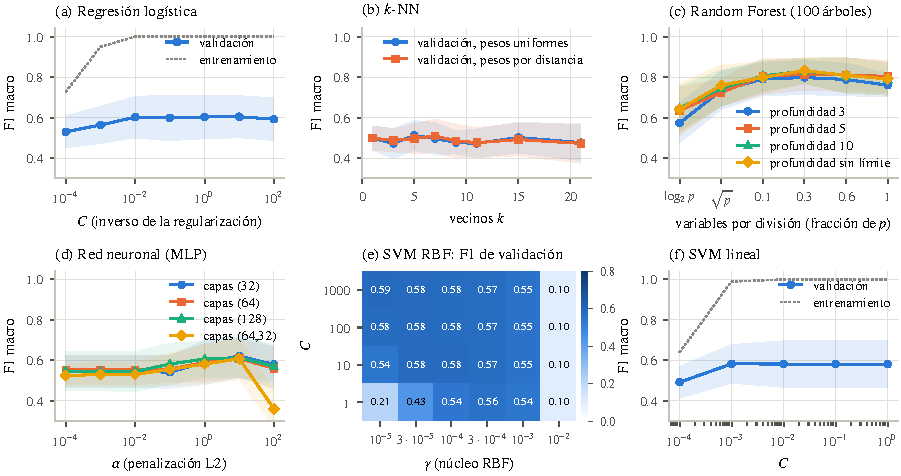
\includegraphics[width=\textwidth]{fig_hyper}
\caption{Efecto de los hiperparámetros sobre el F1 macro de validación (media de 15 particiones sin fuga; banda: IC del 95\,\% de Nadeau--Bengio). (a) Regresión logística. (b) $k$-NN. (c) Random Forest con 100 árboles, por profundidad máxima. (d) MLP, por arquitectura de las capas ocultas. (e) SVM con núcleo RBF (cada celda es el F1 de validación). (f) SVM lineal. Línea punteada: F1 de entrenamiento.}
\label{fig:hyper}
\end{figure*}

\emph{Regresión logística} (Fig.~\ref{fig:hyper}a). Con regularización fuerte ($C=10^{-4}$) el F1 es \N{lr-f1-cmin}; desde $C=10^{-2}$ se estabiliza en torno a \N{lr-f1-c2}, mientras que el F1 de entrenamiento llega a 1.00: el modelo memoriza el entrenamiento porque $p\gg n$.
\emph{$k$-NN} (b). Ni $k$ ni el tipo de pesos cambian el resultado de forma apreciable (F1 entre \N{knn-f1-min} y \N{knn-f1-max}): la distancia euclídea en 1835 dimensiones queda dominada por las 1764 variables HOG, poco discriminantes (Sección~\ref{sec:red}).
\emph{Random Forest} (c). El hiperparámetro decisivo es el número de variables por división: el F1 pasa de \N{rf-f1-log2} con $\log_2p$ a \N{rf-f1-m03} con $0.3p$. La razón es que solo el \N{ind-compact-pct}\,\% de las variables (las 71 no HOG) es informativo: la probabilidad de que un nodo vea al menos una de ellas es \N{rf-see-log2} con $\log_2p$ ($\N{rf-mtry-log2}$ variables), \N{rf-see-sqrt} con $\sqrt p$ y casi 1 con $0.3p$. Con todas las variables el F1 baja a \N{rf-f1-m10} (árboles más correlacionados). La profundidad influye poco (profundidad 3: \N{rf-f1-d3}; sin límite: \N{rf-f1-dinf}) y 300 árboles no mejoran a 100 (\N{rf-f1-n300} frente a \N{rf-f1-n100}).
\emph{MLP} (d). Lo que importa es la penalización L2: con $\alpha\le10^{-2}$ el F1 es \N{mlp-f1-a4}; el óptimo es $\alpha=10$ (\N{mlp-f1-a10}) y con $\alpha=100$ la red subajusta (hasta \N{mlp-f1-a100-min} para (64,32)). La arquitectura casi no influye.
\emph{SVM} (e, f). Con núcleo RBF, $\gamma=10^{-2}$ colapsa el F1 a \N{svm-g1e2} (la matriz de núcleo tiende a la identidad y el modelo predice una sola clase), y $C$ y $\gamma$ pequeños subajustan (\N{svm-c1-g1e5}); en el resto hay una meseta de \N{svm-rbf-plateau-lo} a \N{svm-rbf-plateau-hi}. El núcleo lineal se estabiliza desde $C=10^{-3}$ (\N{svm-lin-best}), sin ventaja del RBF.

\subsection{Desempeño de los modelos: entrenamiento, validación y prueba}\label{sec:desemp}
La Tabla~\ref{tab:res} compara los cinco modelos con su mejor configuración. El Random Forest es el mejor en validación (F1 \N{rf-val-f1}$\pm$\N{rf-val-f1-ci}); su ventaja sobre el segundo, el MLP (\N{mlp-val-f1}$\pm$\N{mlp-val-f1-ci}), es de \N{rf-vs-mlp} puntos de F1 (IC del 95\,\% de la diferencia pareada: $\pm$\N{rf-vs-mlp-ci}), así que es estadísticamente significativa. Los IC del MLP, la regresión logística y la SVM se solapan ampliamente (las diferencias pareadas entre ellos no son concluyentes) y $k$-NN es el peor. Todos los modelos salvo $k$-NN alcanzan un F1 de entrenamiento de 1.00 frente a $\le$\N{rf-val-f1} en validación: sobreajuste que la regularización de las mallas no elimina. En prueba, el Random Forest obtiene exactitud \N{rf-test-acc} [\N{rf-test-acc-lo}, \N{rf-test-acc-hi}] y F1 \N{rf-test-f1} [\N{rf-test-f1-lo}, \N{rf-test-f1-hi}], compatibles con la validación (la exactitud de validación, \N{rf-val-acc}, cae dentro del intervalo), y el orden de los cinco modelos se conserva. Con solo 36 imágenes los IC de Wilson miden cerca de $\pm0.13$ y se solapan entre modelos; por eso la jerarquía se apoya en la validación (204 imágenes $\times$ 15 particiones) y la prueba se usa como confirmación.

\begin{table*}[!t]
\caption{Desempeño de los cinco modelos con su mejor configuración. Validación: media $\pm$ IC del 95\,\% (Nadeau--Bengio, 15 particiones sin fuga). Prueba: 36 imágenes nunca usadas; IC de Wilson (exactitud) y \emph{bootstrap} (F1). Las dos últimas columnas repiten la validación con fuga (copias aumentadas repartidas al azar) y sin aumentación}
\label{tab:res}
\centering\footnotesize
\setlength{\tabcolsep}{2.7pt}\renewcommand{\arraystretch}{1.08}
\begin{tabular}{@{}l >{\raggedright\arraybackslash}p{3.0cm} c c c c c c c c@{}}
\toprule
 & & \multicolumn{2}{c}{Entrenamiento} & \multicolumn{2}{c}{Validación (sin fuga)} & \multicolumn{2}{c}{Prueba ($N=36$)} & \multicolumn{2}{c}{F1 de validación} \\
\cmidrule(lr){3-4}\cmidrule(lr){5-6}\cmidrule(lr){7-8}\cmidrule(l){9-10}
Modelo & Hiperparámetros óptimos & Exactitud & F1 & Exactitud & F1 macro & Exactitud [IC 95\,\%] & F1 macro [IC 95\,\%] & con fuga & sin aument. \\
\midrule
Random Forest & 100 árboles, sin límite, 0.3$p$ var./div. & 1.00 & 1.00 & 0.834$\pm$0.059 & 0.832$\pm$0.063 & 0.778 [0.62, 0.88] & 0.779 [0.62, 0.90] & 0.883 & 0.773 \\
MLP & capas (32), $\alpha=10$ & 1.00 & 1.00 & 0.626$\pm$0.102 & 0.622$\pm$0.106 & 0.667 [0.50, 0.80] & 0.659 [0.48, 0.80] & 0.716 & 0.591 \\
Regresión logística & $C=10$ & 1.00 & 1.00 & 0.610$\pm$0.102 & 0.604$\pm$0.104 & 0.639 [0.48, 0.78] & 0.640 [0.46, 0.78] & 0.710 & 0.585 \\
SVM & RBF, $C=1000$, $\gamma=10^{-5}$ & 1.00 & 1.00 & 0.592$\pm$0.106 & 0.586$\pm$0.108 & 0.528 [0.37, 0.68] & 0.522 [0.34, 0.67] & 0.745 & 0.561 \\
k-NN & $k=5$, pesos uniformes & 0.74 & 0.74 & 0.518$\pm$0.071 & 0.512$\pm$0.074 & 0.472 [0.32, 0.63] & 0.460 [0.29, 0.60] & 0.556 & 0.520 \\
\bottomrule
\end{tabular}
\end{table*}


\begin{figure}[!t]
\centering
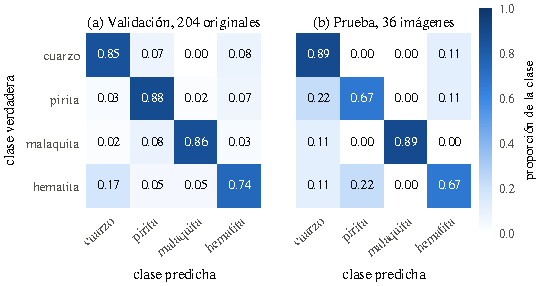
\includegraphics[width=\columnwidth]{fig_confusion}
\caption{Matrices de confusión del Random Forest, normalizadas por clase verdadera (la diagonal es el \emph{recall}). (a) Validación: predicciones fuera de muestra de las 204 imágenes originales (51 por clase, promedio de las 3 repeticiones). (b) Prueba: 36 imágenes (9 por clase).}
\label{fig:cm}
\end{figure}

La Fig.~\ref{fig:cm} muestra qué minerales se confunden. La hematita es la clase más difícil en validación (\emph{recall} \N{cmv-3-3}; se confunde con el cuarzo en \N{cmv-3-0} de los casos) y la malaquita la más fácil en prueba (precisión \N{tpc-p-2}, \emph{recall} \N{tpc-r-2}); en prueba, la pirita y la hematita tienen un \emph{recall} de \N{tpc-r-1} y \N{tpc-r-3}, es decir, 3 de las 9 imágenes de cada clase fallan (una cifra que, con $N=9$, es muy imprecisa).

\subsection{Efecto de la fuga de información y de la aumentación}\label{sec:fuga}
Para cuantificar la fuga se repitió la validación mezclando al azar las 360 filas de entrenamiento (originales y copias), como en el trabajo previo \cite{repo} (penúltima columna de la Tabla~\ref{tab:res}). El F1 sube a \N{rf-naive-f1} para el Random Forest y a \N{svm-naive-f1} para la SVM, frente a \N{rf-val-f1} y \N{svm-val-f1} sin fuga (optimismo de \N{rf-leak-gap} y \N{svm-leak-gap}), y solo la validación sin fuga concuerda con la prueba (F1 de \N{rf-test-f1} y \N{svm-test-f1}). Con la validación sin fuga se puede además medir el efecto de la aumentación (última columna): mejora el F1 del Random Forest en \N{rf-aug-gain}$\pm$\N{rf-aug-gain-ci} (diferencia pareada, IC del 95\,\%), y en los otros cuatro modelos la diferencia no es concluyente (sus IC incluyen el cero; p.~ej., MLP: $\N{mlp-aug-gain}\pm\N{mlp-aug-gain-ci}$).

%% =========================================================================== V
\section{Reducción de dimensión}\label{sec:red}
\subsection{Análisis individual de las variables}\label{sec:ind}
Con las 204 originales de desarrollo (sin las copias, que no son independientes, ni la prueba) se calculó, para cada variable, el índice de discriminación $\eta^2=SS_B/SS_T$ (razón de correlación: fracción de su varianza explicada por la clase; equivale al estadístico $F$ del ANOVA de un factor reescalado a $[0,1]$), su valor $p$ corregido por comparaciones múltiples con el procedimiento de Benjamini--Hochberg \cite{benjamini1995} ($q<0.05$) y la información mutua con la clase, cuyo orden coincide solo en parte con el de $\eta^2$ (Spearman \N{ind-spearman}). Una variable se marca como \emph{redundante} si su correlación absoluta con otra más discriminante ya conservada es $\ge0.95$ (hay \N{ind-pairs} pares así). La Tabla~\ref{tab:ind} y la Fig.~\ref{fig:ind} resumen el resultado.

\begin{table}[!t]
\caption{Análisis individual de las variables por familia: índice de discriminación $\eta^2$ (204 originales), porcentaje de variables significativas ($q<0.05$, Benjamini--Hochberg) y candidatas a eliminar (no significativas o redundantes, $|\rho|\ge0.95$)}
\label{tab:ind}
\centering\footnotesize
\setlength{\tabcolsep}{2.6pt}\renewcommand{\arraystretch}{1.05}
\begin{tabular}{@{}l r c c r r r r@{}}
\toprule
Familia & $n$ & $\tilde\eta^2$ & $\eta^2_{\max}$ & \% sig. & Redund. & Candid. & Conserv.\\
\midrule
HOG & 1764 & 0.042 & 0.238 & 46 & 142 & 1096 & 668\\
Color & 18 & 0.205 & 0.515 & 100 & 3 & 3 & 15\\
Gabor & 16 & 0.203 & 0.255 & 100 & 11 & 11 & 5\\
LBP & 10 & 0.275 & 0.322 & 100 & 4 & 4 & 6\\
GLCM & 20 & 0.303 & 0.399 & 100 & 10 & 10 & 10\\
Hu & 7 & 0.123 & 0.134 & 71 & 4 & 6 & 1\\
\midrule
Total & 1835 & 0.044 & 0.515 & 48 & 174 & 1130 & 705\\
\bottomrule
\end{tabular}
\end{table}


\begin{figure}[!t]
\centering
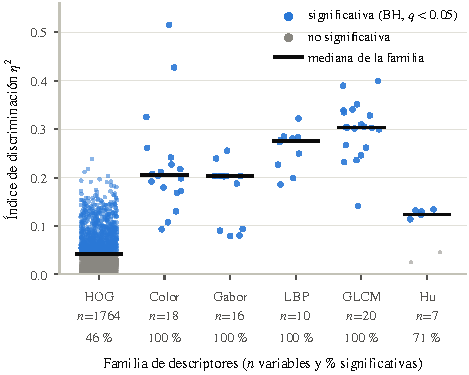
\includegraphics[width=\columnwidth]{fig_individual}
\caption{Índice de discriminación $\eta^2$ de las 1835 variables por familia de descriptores (un punto por variable; en HOG, 1764 puntos). Azul: significativa (Benjamini--Hochberg, $q<0.05$); gris: no significativa; trazo negro: mediana de la familia.}
\label{fig:ind}
\end{figure}

La información está concentrada: las 71 variables no HOG (\N{ind-compact-pct}\,\% del total) son casi todas significativas, con $\eta^2$ mediana entre \N{ind-hu-eta} (Hu) y \N{ind-glcm-eta} (GLCM); la mayor es la asimetría del canal $a^*$ de CIELAB ($\eta^2=\N{ind-top-eta}$), y solo \N{ind-top50-hog} de las 50 variables con mayor $\eta^2$ son HOG. De las 1764 variables HOG, en cambio, solo el \N{ind-hog-pct}\,\% es significativa (mediana \N{ind-hog-eta}, máximo \N{ind-hog-etamax}). Son \emph{candidatas a eliminar} \N{ind-cand} variables (\N{ind-pct-cand}\,\%): \N{ind-nonsig} no significativas (954 HOG y 2 Hu) y \N{ind-red} significativas pero redundantes. La redundancia es estructural: las 8 medias de Gabor son prácticamente idénticas entre sí y a la luminancia media (\mbox{$|\rho|\approx1$}), la energía GLCM es igual en tres ángulos y los momentos de Hu 2--6 están muy correlacionados. Entre las compactas son candidatas, por ejemplo, las tres variables de la luminancia $L^*$, las 8 medias de Gabor, 10 variables de GLCM y los momentos de Hu 1 y 3--7; la lista completa (variable, familia, $\eta^2$, $q$ y marca de candidata) está en \texttt{results/\allowbreak variables\_individual.csv}. Quedan \N{ind-cons} variables. Que una variable sea individualmente poco discriminante no implica que sea inútil en conjunto (las HOG podrían aportar por interacción), así que el efecto real de eliminarlas se mide con los modelos.

\subsection{Selección de variables y criterio para $k$}\label{sec:sel}
Para las tres técnicas se re-evalúan los dos mejores modelos (Random Forest y MLP) con la misma validación sin fuga: la reducción se ajusta en cada pliegue solo con el entrenamiento y cada modelo se re-ajusta en el espacio reducido con una malla pequeña (Random Forest: 300 árboles y $\sqrt k$, $0.3k$ o $k$ variables por división; MLP: 128 neuronas y $\alpha\in\{10^{-2},1,10\}$), con las componentes o variables reestandarizadas. El tamaño $k^*$ se elige con un criterio propio, la \emph{regla de un error estándar} \cite{hastie2009}: el menor $k$ cuyo F1 medio de validación está a menos de un error estándar (el de Nadeau--Bengio) del mejor $k$ de la malla; así se prefiere la representación más pequeña entre las que no son distinguibles de la mejor. Con $k^*$ se reajusta el modelo con todo el desarrollo y se evalúa en la prueba. El \emph{porcentaje de reducción} es $(1835-k^*)/1835$.

\emph{Selección por $\eta^2$ (filtro).} Se conservan las $k$ variables no redundantes con mayor $\eta^2$ (calculado en cada pliegue solo con las originales del entrenamiento), $k\in\{5,\dots,800\}$. Con el Random Forest, $k^*=\N{sel-rf-kstar}$ variables (reducción de \N{sel-rf-red}\,\%) dan F1 \N{sel-rf-val-f1}$\pm$\N{sel-rf-val-f1-ci}, indistinguible de las 1835 (diferencia pareada \N{sel-rf-dif}$\pm$\N{sel-rf-dif-ci}); son \N{sel-rf-comp} variables, todas salvo 3 de las familias compactas. El MLP \emph{mejora}: de \N{mlp-val-f1} a \N{sel-mlp-val-f1}$\pm$\N{sel-mlp-val-f1-ci} con $k^*=\N{sel-mlp-kstar}$ (\N{sel-mlp-comp}; diferencia pareada $+\N{sel-mlp-dif}\pm\N{sel-mlp-dif-ci}$) y su F1 de entrenamiento baja de 1.00 a \N{sel-mlp-trainf1}, es decir, sobreajusta menos al quitar las variables HOG ruidosas. Esto coincide con el análisis individual: conservar \emph{todas} las variables significativas no redundantes (\N{sel-rf-allsig-n} por pliegue, casi todas HOG) ya no ayuda (Random Forest \N{sel-rf-allsig-f1}, MLP \N{sel-mlp-allsig-f1}), porque lo que aporta es el pequeño grupo de descriptores muy discriminantes.

\subsection{Análisis de componentes principales (PCA)}\label{sec:pca}
El PCA \cite{jolliffe2002} se ajusta en cada pliegue con el entrenamiento (variables estandarizadas, 1835 dimensiones, sin usar las etiquetas) y proyecta la validación y la prueba; se exploraron $k\in\{2,3,5,8,12,16,24,32,48,64,96,128\}$ componentes, siempre muchas menos que variables. \emph{Criterio para $k$.} El criterio clásico de varianza explicada pediría \N{pca-k80}, \N{pca-k90} y \N{pca-k95} componentes para retener el 80, 90 y 95\,\% de la varianza; pero lo que interesa conservar no es la varianza sino la separación de las clases, así que se aplica la regla de un error estándar sobre el F1 de validación (Sec.~\ref{sec:sel}) y se reporta la varianza explicada como medida complementaria. No se exploraron más de 128 componentes (\N{pca-var128}\,\% de la varianza) porque el F1 no mejora de forma apreciable desde $k=32$.

Con $k^*=\N{pca-rf-kstar}$ componentes (reducción de \N{pca-rf-red}\,\%; \N{pca-rf-var}\,\% de la varianza) el Random Forest cae a F1 \N{pca-rf-val-f1}$\pm$\N{pca-rf-val-f1-ci} (diferencia pareada con las 1835 variables: $\N{pca-rf-dif}\pm\N{pca-rf-dif-ci}$, significativa) y el MLP a \N{pca-mlp-val-f1}$\pm$\N{pca-mlp-val-f1-ci} ($\N{pca-mlp-dif}\pm\N{pca-mlp-dif-ci}$, no concluyente); ninguno mejora de forma apreciable con más componentes (Fig.~\ref{fig:red}b: el mejor $k$ de la malla da \N{pca-rf-f1best} y \N{pca-mlp-f1best}). En prueba, el F1 es \N{pca-rf-test-f1} [\N{pca-rf-test-f1-lo}, \N{pca-rf-test-f1-hi}] y \N{pca-mlp-test-f1} [\N{pca-mlp-test-f1-lo}, \N{pca-mlp-test-f1-hi}] (Tabla~\ref{tab:red}).

\emph{¿Por qué no ayuda el PCA?} Porque la varianza no es discriminación. Las 71 variables compactas, que son las informativas, aportan solo el \N{pcadiag-compact-var}\,\% de la varianza total y por eso no dominan ninguna de las primeras componentes: en las 32 primeras, el \N{pcadiag-hog-share32}\,\% de la norma de las cargas corresponde a variables HOG (el \N{pcadiag-hog-expected}\,\% si se repartieran por igual). La componente con mayor $\eta^2$ (la primera) alcanza \N{pcadiag-max-eta}, menos de la mitad de la mejor variable individual (\N{ind-top-eta}), y solo \N{pcadiag-n-eta02} de las 128 primeras componentes superan $\eta^2=0.2$, frente a \N{ind-n-eta02} variables individuales. El Random Forest, que divide por una variable a la vez, pierde mucho más que el MLP porque el PCA mezcla cada descriptor útil con cientos de variables HOG, mientras que la primera capa del MLP ya es una combinación lineal de las entradas.

\subsection{UMAP}\label{sec:umap}
UMAP \cite{mcinnes2018} construye un grafo ponderado con los 15 vecinos más cercanos de cada punto (distancia euclídea sobre las 1835 variables estandarizadas) y busca una representación de baja dimensión que lo preserve (\texttt{min\_dist}$=0.1$). Es no supervisado y no tiene un análogo de la varianza explicada, así que $k\in\{2,3,5,8,12,16,24,32\}$ se elige solo con la regla de un error estándar. Se ajusta en cada pliegue con el entrenamiento y la validación y la prueba se proyectan con su función \texttt{transform}. Como \texttt{umap-learn} (y \texttt{numba}) no estaba disponible en el entorno de ejecución, el algoritmo se programó en NumPy siguiendo los pasos y los valores por defecto de la referencia (archivo \texttt{umap\_np.py}); en el conjunto \emph{digits} de scikit-learn, el 5-NN sobre el plano de 2 dimensiones acierta 0.976 (con PCA, 0.606). Con la librería oficial las cifras pueden variar ligeramente.

Con $k^*=\N{umap-rf-kstar}$ dimensiones (reducción de \N{umap-rf-red}\,\%) el Random Forest cae a F1 \N{umap-rf-val-f1}$\pm$\N{umap-rf-val-f1-ci} (diferencia pareada $\N{umap-rf-dif}\pm\N{umap-rf-dif-ci}$) y el MLP, con $k^*=\N{umap-mlp-kstar}$, a \N{umap-mlp-val-f1}$\pm$\N{umap-mlp-val-f1-ci} ($\N{umap-mlp-dif}\pm\N{umap-mlp-dif-ci}$); las dos caídas son significativas. La curva es plana (Fig.~\ref{fig:red}c): con 32 dimensiones el mejor F1 es \N{umap-rf-f1best} (Random Forest) y \N{umap-mlp-f1best} (MLP). En prueba, el F1 es \N{umap-rf-test-f1} [\N{umap-rf-test-f1-lo}, \N{umap-rf-test-f1-hi}] y \N{umap-mlp-test-f1} [\N{umap-mlp-test-f1-lo}, \N{umap-mlp-test-f1-hi}] (Tabla~\ref{tab:red}). La causa es la geometría de la que parte UMAP: de los 15 vecinos más cercanos de una imagen, solo una fracción de \N{nbr-pur-all} pertenece a su misma clase con las 1835 variables (azar: \N{nbr-pur-chance}), frente a \N{nbr-pur-compact} con solo las 71 no HOG. UMAP no puede crear una separación que su grafo no contiene, lo que es coherente con que su desempeño se parezca al de $k$-NN (F1 \N{knn-val-f1}).

\begin{table*}[!t]
\caption{Efecto de la reducción de dimensión sobre los dos mejores modelos. $k^*$: n.º de variables o componentes elegido con la regla de un error estándar sobre el F1 de validación (15 particiones sin fuga, media $\pm$ IC 95\,\%); reducción $=(1835-k^*)/1835$; var.~expl.: varianza explicada acumulada (solo PCA). Con $k^*$ se reajusta con todo el desarrollo y se evalúa en prueba ($N=36$)}
\label{tab:red}
\centering\footnotesize
\setlength{\tabcolsep}{2.8pt}\renewcommand{\arraystretch}{1.08}
\begin{tabular}{@{}l l r r r c c c c c c@{}}
\toprule
 & & & & & \multicolumn{2}{c}{Entrenamiento} & \multicolumn{2}{c}{Validación (sin fuga)} & \multicolumn{2}{c}{Prueba ($N=36$)}\\
\cmidrule(lr){6-7}\cmidrule(lr){8-9}\cmidrule(l){10-11}
Modelo & Representación & $k^*$ & Reducc. (\%) & Var.~expl. (\%) & Exact. & F1 & Exactitud & F1 macro & Exactitud [IC 95\,\%] & F1 macro [IC 95\,\%]\\
\midrule
Random Forest & Todas las variables & 1835 & 0.0 & -- & 1.00 & 1.00 & 0.834$\pm$0.059 & 0.832$\pm$0.063 & 0.778 [0.62, 0.88] & 0.779 [0.62, 0.90] \\
 & Selección por $\eta^2$ & 30 & 98.4 & -- & 1.00 & 1.00 & 0.835$\pm$0.062 & 0.833$\pm$0.066 & 0.750 [0.59, 0.86] & 0.750 [0.59, 0.88] \\
 & PCA & 32 & 98.3 & 53.9 & 1.00 & 1.00 & 0.528$\pm$0.061 & 0.523$\pm$0.066 & 0.611 [0.45, 0.75] & 0.606 [0.43, 0.73] \\
 & UMAP & 8 & 99.6 & -- & 1.00 & 1.00 & 0.477$\pm$0.099 & 0.468$\pm$0.104 & 0.500 [0.34, 0.66] & 0.497 [0.32, 0.64] \\
\midrule
MLP & Todas las variables & 1835 & 0.0 & -- & 1.00 & 1.00 & 0.626$\pm$0.102 & 0.622$\pm$0.106 & 0.667 [0.50, 0.80] & 0.659 [0.48, 0.80] \\
 & Selección por $\eta^2$ & 10 & 99.5 & -- & 0.92 & 0.92 & 0.786$\pm$0.100 & 0.782$\pm$0.111 & 0.750 [0.59, 0.86] & 0.745 [0.58, 0.87] \\
 & PCA & 32 & 98.3 & 53.9 & 0.83 & 0.83 & 0.559$\pm$0.067 & 0.552$\pm$0.074 & 0.444 [0.30, 0.60] & 0.439 [0.26, 0.59] \\
 & UMAP & 3 & 99.8 & -- & 0.60 & 0.60 & 0.474$\pm$0.091 & 0.467$\pm$0.091 & 0.556 [0.40, 0.70] & 0.556 [0.37, 0.70] \\
\bottomrule
\end{tabular}
\end{table*}


\begin{figure*}[!t]
\centering
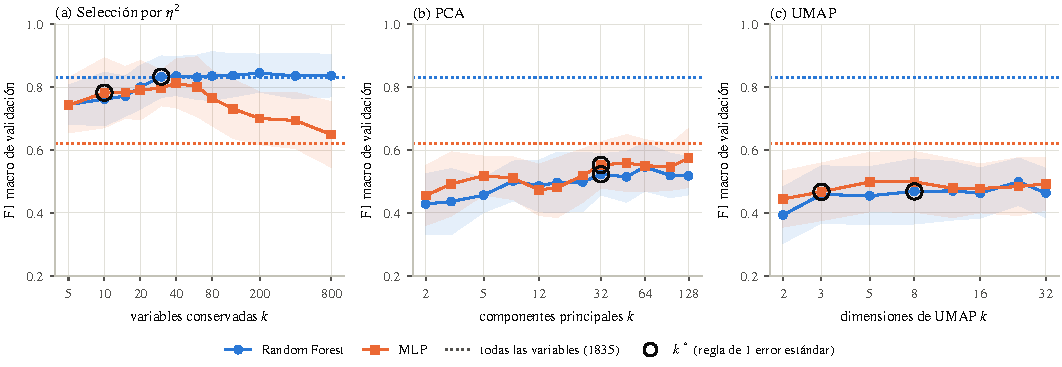
\includegraphics[width=\textwidth]{fig_reduction}
\caption{F1 macro de validación en función del tamaño de la representación $k$ para los dos mejores modelos (media de 15 particiones sin fuga; banda: IC del 95\,\% de Nadeau--Bengio). (a) Selección por $\eta^2$. (b) PCA. (c) UMAP. Línea punteada: F1 con las 1835 variables; círculo: $k^*$ elegido con la regla de un error estándar.}
\label{fig:red}
\end{figure*}

\subsection{Comparación y discusión}\label{sec:comp}
La Tabla~\ref{tab:red} y la Fig.~\ref{fig:red} comparan las tres técnicas con la línea base de 1835 variables. Para los dos modelos el orden es el mismo: selección por $\eta^2$ $\gtrsim$ todas las variables $>$ PCA $\gtrsim$ UMAP. La selección supera a PCA en \N{sel-pca-rf}$\pm$\N{sel-pca-rf-ci} puntos de F1 con el Random Forest y en \N{sel-pca-mlp}$\pm$\N{sel-pca-mlp-ci} con el MLP, y a UMAP en \N{sel-umap-rf}$\pm$\N{sel-umap-rf-ci} y \N{sel-umap-mlp}$\pm$\N{sel-umap-mlp-ci} (diferencias pareadas, todas significativas); entre PCA y UMAP la diferencia es pequeña (Random Forest: \N{pca-umap-rf}$\pm$\N{pca-umap-rf-ci}; MLP: \N{pca-umap-mlp}$\pm$\N{pca-umap-mlp-ci}).

\emph{Causa común.} Las tres técnicas reducen más del 98\,\% de la dimensión, pero solo la selección usa las etiquetas. Como el \N{pcadiag-hog-expected}\,\% de las variables es HOG, la varianza (PCA) y la vecindad euclídea (UMAP) quedan dominadas por ellas, mientras que la información sobre la clase está en las 71 variables compactas (Sec.~\ref{sec:ind}): el filtro por $\eta^2$ las encuentra directamente, y PCA y UMAP, al ser no supervisados, las diluyen. La Fig.~\ref{fig:emb} lo ilustra: en ambas proyecciones de 2 dimensiones las cuatro clases se solapan.

\begin{figure*}[!t]
\centering
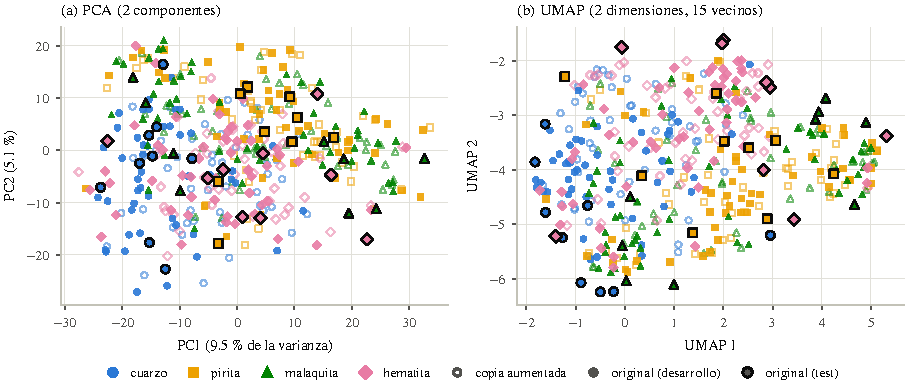
\includegraphics[width=\textwidth]{fig_embed}
\caption{Proyecciones de 2 dimensiones del conjunto de desarrollo y de la prueba, coloreadas por clase. (a) PCA. (b) UMAP (15 vecinos, \texttt{min\_dist}$=0.1$). Los puntos huecos son copias aumentadas; los de borde negro, imágenes de prueba proyectadas con el modelo ajustado solo con el desarrollo.}
\label{fig:emb}
\end{figure*}

\emph{Modelo recomendado.} Si se busca el modelo más sencillo sin perder desempeño, la mejor opción es el Random Forest con las \N{sel-rf-kstar} variables de mayor $\eta^2$ (\N{sel-rf-comp}: solo \N{sel-rf-nhog} son HOG), que iguala a las 1835 variables en validación (\N{sel-rf-val-f1} frente a \N{rf-val-f1}) y en prueba (exactitud \N{sel-rf-test-acc} [\N{sel-rf-test-acc-lo}, \N{sel-rf-test-acc-hi}] frente a \N{rf-test-acc} [\N{rf-test-acc-lo}, \N{rf-test-acc-hi}]), con una reducción de \N{sel-rf-red}\,\%. El MLP pasa de \N{mlp-val-f1} a \N{sel-mlp-val-f1} con solo \N{sel-mlp-kstar} variables, pero sigue por debajo del Random Forest y con IC muy anchos.

%% =========================================================================== VI
\section{Conclusiones}
\emph{Objetivos.} (O1) Se caracterizó la base (432 filas $\times$ 1835 variables numéricas, sin datos faltantes, cuatro clases balanceadas) y se justificó el aprendizaje supervisado. (O2) Se compararon cinco modelos con \N{ncfg-total} configuraciones de hiperparámetros: el Random Forest es el mejor (F1 de validación \N{rf-val-f1}$\pm$\N{rf-val-f1-ci}; exactitud en prueba \N{rf-test-acc}, IC del 95\,\% [\N{rf-test-acc-lo}, \N{rf-test-acc-hi}]), porque solo el \N{ind-compact-pct}\,\% de las variables es informativo y las 1764 HOG perjudican a los modelos que usan todas las variables por igual. (O3) La reducción supervisada por $\eta^2$ conserva el desempeño con \N{sel-rf-kstar} variables (\N{sel-rf-red}\,\% menos) y mejora al MLP, mientras que PCA y UMAP, no supervisados, lo degradan de forma significativa.

\emph{Hallazgos metodológicos.} La validación con fuga de información sobreestima el F1 hasta \N{svm-leak-gap} puntos y no concuerda con la prueba; la aumentación solo mejora de forma significativa al Random Forest (\N{rf-aug-gain}$\pm$\N{rf-aug-gain-ci}); y reportar intervalos de confianza evita sobreinterpretar diferencias que no son concluyentes (el efecto de la aumentación en los otros cuatro modelos, o el del MLP frente a la regresión logística y la SVM).

\emph{Limitaciones.} (i) La prueba tiene 36 imágenes y sus IC miden cerca de $\pm0.13$, por lo que las decisiones se apoyan en la validación (204 imágenes $\times$ 15 particiones). (ii) Las imágenes de prueba provienen de la misma fuente que las de entrenamiento y no se verificó si el banco contiene imágenes casi duplicadas, de modo que el desempeño con fotografías de otro origen puede ser menor (en \cite{long2025} cae de 90.7 a 80.2\,\%). (iii) Los hiperparámetros y $k^*$ se eligen con la misma validación con la que se reportan, lo que produce un optimismo leve \cite{cawley2010}; la prueba sirve de contraste. (iv) UMAP se ejecutó con una implementación propia.

\emph{Trabajo futuro.} Medir el cambio de dominio con un conjunto de prueba propio (fotografías de otro dispositivo); reemplazar HOG por incrustaciones de una red convolucional preentrenada; y comparar el filtro por $\eta^2$ con métodos supervisados de reducción (importancia del Random Forest, PLS-DA, UMAP supervisado).

\emph{Disponibilidad.} El código, los resultados guardados y el cuaderno que reproduce todas las tablas y figuras de este informe están en \expandafter\url\expandafter{\REPOURL}.

%% =========================================================================== Referencias
\begin{thebibliography}{99}
\bibitem{chow2022} B. H. Y. Chow and C. C. Reyes-Aldasoro, ``Automatic gemstone classification using computer vision,'' \emph{Minerals}, vol. 12, no. 1, Art. 60, 2022, doi: 10.3390/min12010060.
\bibitem{zeng2021} X. Zeng, Y. Xiao, X. Ji, and G. Wang, ``Mineral identification based on deep learning that combines image and Mohs hardness,'' \emph{Minerals}, vol. 11, no. 5, Art. 506, 2021, doi: 10.3390/min11050506.
\bibitem{hfdata} tedqc, ``mineral-dataset,'' Hugging Face Datasets, 2025. [Online]. Available: \url{https://huggingface.co/datasets/tedqc/mineral-dataset}
\bibitem{repo} Mista299, ``clasificador-minerales-pdi-udea-2026-2,'' repositorio de GitHub (Procesamiento Digital de Im\'agenes, Universidad de Antioquia), 2026. [Online]. Available: \url{https://github.com/Mista299/clasificador-minerales-pdi-udea-2026-2}
\bibitem{dalal2005} N. Dalal and B. Triggs, ``Histograms of oriented gradients for human detection,'' in \emph{Proc. IEEE Conf. Comput. Vis. Pattern Recognit. (CVPR)}, 2005, vol. 1, pp. 886--893.
\bibitem{ojala2002} T. Ojala, M. Pietik\"ainen, and T. M\"aenp\"a\"a, ``Multiresolution gray-scale and rotation invariant texture classification with local binary patterns,'' \emph{IEEE Trans. Pattern Anal. Mach. Intell.}, vol. 24, no. 7, pp. 971--987, Jul. 2002.
\bibitem{haralick1973} R. M. Haralick, K. Shanmugam, and I. Dinstein, ``Textural features for image classification,'' \emph{IEEE Trans. Syst., Man, Cybern.}, vol. SMC-3, no. 6, pp. 610--621, Nov. 1973.
\bibitem{hu1962} M.-K. Hu, ``Visual pattern recognition by moment invariants,'' \emph{IRE Trans. Inf. Theory}, vol. 8, no. 2, pp. 179--187, Feb. 1962.
\bibitem{maitre2019} J. Maitre, K. Bouchard, and L. P. Bédard, ``Mineral grains recognition using computer vision and machine learning,'' \emph{Comput. Geosci.}, vol. 130, pp. 84--93, 2019, doi: 10.1016/j.cageo.2019.05.009.
\bibitem{liu2019} C. Liu, M. Li, Y. Zhang, S. Han, and Y. Zhu, ``An enhanced rock mineral recognition method integrating a deep learning model and clustering algorithm,'' \emph{Minerals}, vol. 9, no. 9, Art. 516, 2019, doi: 10.3390/min9090516.
\bibitem{zhang2019} Y. Zhang, M. Li, S. Han, Q. Ren, and J. Shi, ``Intelligent identification for rock-mineral microscopic images using ensemble machine learning algorithms,'' \emph{Sensors}, vol. 19, no. 18, Art. 3914, 2019, doi: 10.3390/s19183914.
\bibitem{jia2021} L. Jia, M. Yang, F. Meng, M. He, and H. Liu, ``Mineral photos recognition based on feature fusion and online hard sample mining,'' \emph{Minerals}, vol. 11, no. 12, Art. 1354, 2021, doi: 10.3390/min11121354.
\bibitem{long2025} B. Long and C. Zhou, ``Enhanced mineral image classification using YOLOv8-CLS with optimized feature extraction and dataset augmentation,'' \emph{Informatica}, vol. 49, no. 34, pp. 87--108, 2025, doi: 10.31449/inf.v49i34.7927.
\bibitem{nadeau2003} C. Nadeau and Y. Bengio, ``Inference for the generalization error,'' \emph{Mach. Learn.}, vol. 52, no. 3, pp. 239--281, 2003.
\bibitem{wilson1927} E. B. Wilson, ``Probable inference, the law of succession, and statistical inference,'' \emph{J. Amer. Statist. Assoc.}, vol. 22, no. 158, pp. 209--212, 1927.
\bibitem{efron1993} B. Efron and R. J. Tibshirani, \emph{An Introduction to the Bootstrap}. New York, NY, USA: Chapman \& Hall, 1993.
\bibitem{breiman2001} L. Breiman, ``Random forests,'' \emph{Mach. Learn.}, vol. 45, no. 1, pp. 5--32, 2001.
\bibitem{cortes1995} C. Cortes and V. Vapnik, ``Support-vector networks,'' \emph{Mach. Learn.}, vol. 20, no. 3, pp. 273--297, 1995.
\bibitem{sklearn2011} F. Pedregosa \emph{et al.}, ``Scikit-learn: Machine learning in Python,'' \emph{J. Mach. Learn. Res.}, vol. 12, pp. 2825--2830, 2011.
\bibitem{benjamini1995} Y. Benjamini and Y. Hochberg, ``Controlling the false discovery rate: A practical and powerful approach to multiple testing,'' \emph{J. R. Stat. Soc. Ser. B}, vol. 57, no. 1, pp. 289--300, 1995.
\bibitem{hastie2009} T. Hastie, R. Tibshirani, and J. Friedman, \emph{The Elements of Statistical Learning}, 2nd ed. New York, NY, USA: Springer, 2009.
\bibitem{jolliffe2002} I. T. Jolliffe, \emph{Principal Component Analysis}, 2nd ed. New York, NY, USA: Springer, 2002.
\bibitem{mcinnes2018} L. McInnes, J. Healy, and J. Melville, ``UMAP: Uniform manifold approximation and projection for dimension reduction,'' arXiv:1802.03426, 2018.
\bibitem{cawley2010} G. C. Cawley and N. L. C. Talbot, ``On over-fitting in model selection and subsequent selection bias in performance evaluation,'' \emph{J. Mach. Learn. Res.}, vol. 11, pp. 2079--2107, 2010.
\end{thebibliography}
\end{document}
